\section{Additional Optimizations}
\label{sec:opts}

While our implementation does not yet map a declarative Brados specification
to a particular physical design, the specification provides a powerful
infrastructure for automating this mapping and achieving other optimizations.

\subsection{Batching}

Figure~\ref{fig:batching} shows the performance benefits of batching log
appends for two different implementations. The \emph{simple} implementation
uses internal I/O interfaces to process each append independently, and the
modest performance benefits are due to the amatorization of the fixed
per-request cost. The \emph{batch-aware} implementation is able to achieve much
higher performance by constructing more efficient I/O requests using range
queries and data sieving.

\begin{figure}
\centering
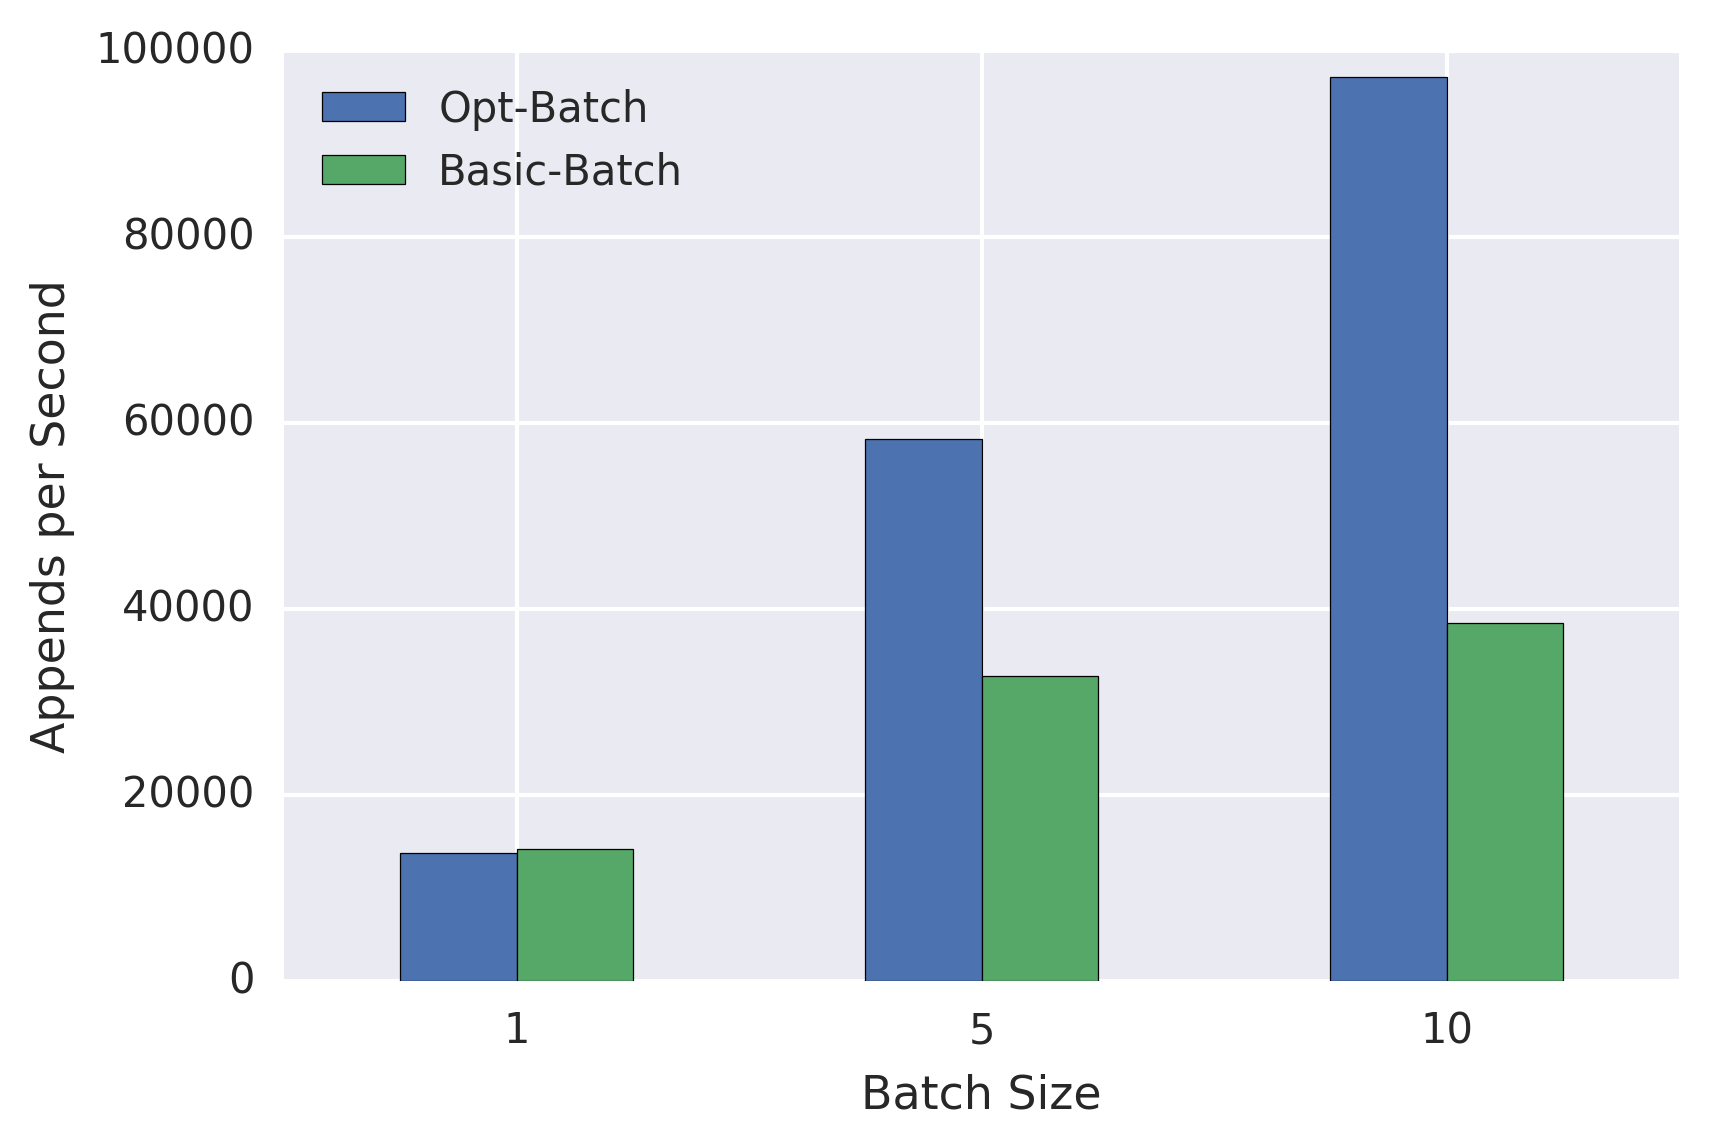
\includegraphics[width=1.0\linewidth]{batching.png}
\caption{Total throughput with and without batching.}
\label{fig:batching}
\end{figure}

While the performance impact of application-specific batching is significant,
techniques such as range queries and data sieving are sensitive to outliers.
For example, handling two requests independently will become more efficient
than using a data sieving technique as the size of the range between the
requests increases. Figure~\ref{fig:batching-outlier} highlights this
challenge. The \emph{simple} implementation has consistent, but relatively
worse performance. The \emph{batch-aware} implementation achieves high append
throughput, but performance degrades as the magnitude of the batch outlier
increases. In contrast, the \emph{batch-oident} applies a simple heuristic to
identify the outlier and handle it independently, resulting in only a slight
decrease in performance over the best case.

\begin{figure}
\centering
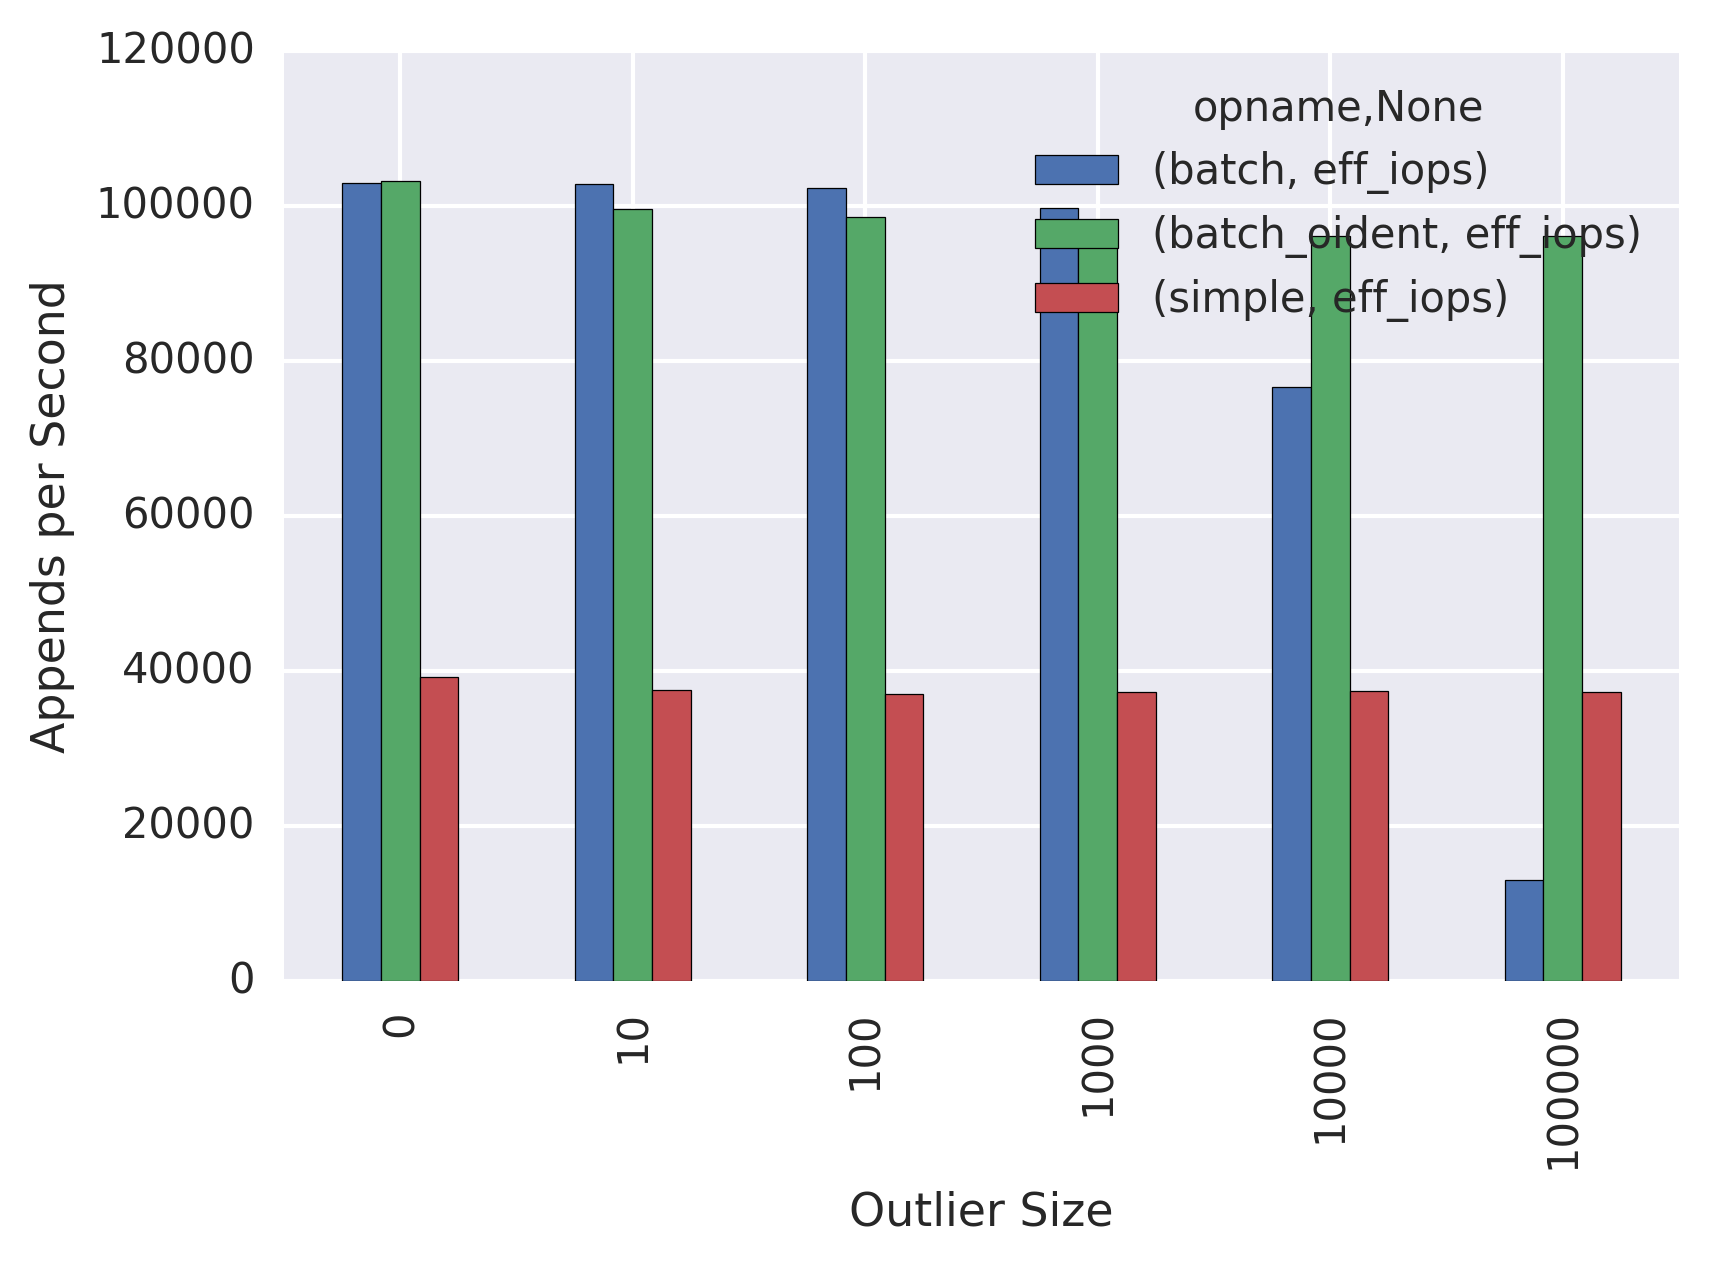
\includegraphics[width=1.0\linewidth]{batching-outlier-detect.png}
\caption{Identifying and handling an outlier independently maintains the
beneifts of batching without the performance degredation of unecessarily
large I/O requests.}
\label{fig:batching-outlier}
\end{figure}

\subsection{Physical Design}

The challenge of navigating the physical design space
has served as the primary source of motivation for selection of a declarative
language. Given the declarative nature of the interfaces we have defined,
we can draw parallels between the physical design challenges described in this
paper and the
large body of mature work in query planning and optimization. Consider the
simple interface reference counting interface described in
Section~\ref{sec:oi}.  The C++ interface makes a strong assumption about a
relatively small number of tags, and chooses to fully serialize and
deserialize a C++ \texttt{std::map} for every request and store the marshalled
data as an extended attribute.  As the number of tags grows the cost of false
sharing will increase to the point that selection of an index-based interface
will likely offer a performance advantage. While the monolithic version can
outperform for small sets of tags, this type of optimization decision is
precisely what can be achieved using a declarative interface definition that
hides low-level evaluation aspects such as physical design.

Looking beyond standard forms of optimization decisions that seek to select
an appropriate mix of low-level I/O interfaces, data structure selection is an
important point of optimization. For instance in Section~\ref{sec:mm} we
showed that using the bytestream for metadata management as opposed to the
key-value interface offered superior performance. However the unstructured
nature of the bytestream data model imposes no restrictions on implementation
or storage layout. Integration of common indexing techniques into an optimizer
combined with a performance model will allow our CORFU interface to derive
similar optimizations when appropriate.

\subsection{Static Analysis}

The Bloom language that we use as a basis for Brados
produces a data flow graph that can be used in static analysis. We envision
that this graph will be made available to the OSD and used to reorder and
coalesce requests based on optimization criteria available from a performance
model combined with semantic information from the dataflow. For example today
object classes are represented as black boxes from the point of view of the
OSD execution engine.  Understanding the behavior of an object class may allow
intelligent prefetching. Another type of analysis that may be useful for
optimization is optimistic execution combined with branch prediction where
frequent paths through a dataflow are handled optimistically.
